\newcommand*{\PathToAssets}{../assets}%
\newcommand*{\PathToOutput}{../output}%
\documentclass{article}
\usepackage[a4paper, margin=1in]{geometry}
\usepackage{graphicx}
\usepackage{caption}
\usepackage{float}
\usepackage{booktabs}

\title{Replication Report}
\author{Aadi Deshpande}
\date{\today}

\begin{document}

\maketitle

\section{Introduction}
This report summarizes the process of retrieving, preprocessing, and analyzing financial data from multiple sources. Additionally, it presents a replication of key tables and figures from the referenced research paper. Specifically, we focus on \textbf{Table 1}, \textbf{Table 1A}, and \textbf{Figure 1A} from the paper, detailing the methodology behind their generation and comparing our reproduced results.

\section{Replication of Research Findings}

\subsection{Table 1: Mark-to-Market Statistics by Bank Size}
Table 1 presents descriptive statistics of key metrics after marking to market the asset values for FDIC-insured depository institutions in the United States. The methodology involved:

\begin{itemize}
    \item Retrieving Q1 2022 balance sheet data from \textbf{bank call reports}.
    \item Marking to market all securities and loans using \textbf{market price growth from Q1 2022 to Q1 2023}.
    \item Calculating the aggregate loss, loss percentage by asset type, and uninsured deposit exposure.
\end{itemize}

\subsection{Table 1A: Bank Balance Sheets}
Table 1A provides an overview of bank asset compositions, liabilities, and equity distributions. The methodology involved:

\begin{itemize}
    \item Defining four bank categories: \textbf{small banks, large banks (non-GSIB), GSIB banks, and the aggregate sample}.
    \item Extracting financial compositions, including cash holdings, securities, real estate loans, and other assets.
    \item Normalizing data by \textbf{winsorizing at the 5th and 95th percentiles}.
    \item Computing summary statistics with mean values and standard deviations.
\end{itemize}

\subsection{Figure 1A: Aggregate Bank Assets and Liabilities}
Figure 1A plots the composition of aggregate total assets and liabilities of U.S. banks as of Q1 2022 in trillions of dollars (see also Table A1). On the asset side, banks had about \$24 trillion of assets as of Q1 2022. Of these:

\begin{itemize}
    \item \textbf{Cash} constitutes about 14\% of aggregate bank assets.
    \item \textbf{Security}, which includes bank investments in U.S. Treasurys, RMBS, CMBS, ABS, and other securities, accounts for about 25\%.
    \item \textbf{Real Estate Loan}, including residential and commercial loans, accounts for 22\%.
    \item \textbf{Other Loan}, which includes commercial and industrial loans, consumer loans, and agricultural loans, accounts for 20\%.
    \item \textbf{Other Asset} accounts for the remaining bank assets.
\end{itemize}

On the liability side:

\begin{itemize}
    \item \textbf{Insured Deposits} account for about 41\% of total bank funding.
    \item \textbf{Uninsured Deposits} account for about 37\% (approximately \$9 trillion).
    \item \textbf{Other} includes loans and liabilities.
    \item \textbf{Equity} accounts for about 9.5\% of total bank liabilities.
\end{itemize}

Data sources: Bank call reports.

\section{Comparison of Replication Results}
To compare our replicated results with the original paper, we present the original results as a figure (provided as a PNG) and our computed values as a table.

\subsection{Original Table 1 (Extracted from Paper)}
\begin{figure}[H]
    \centering
    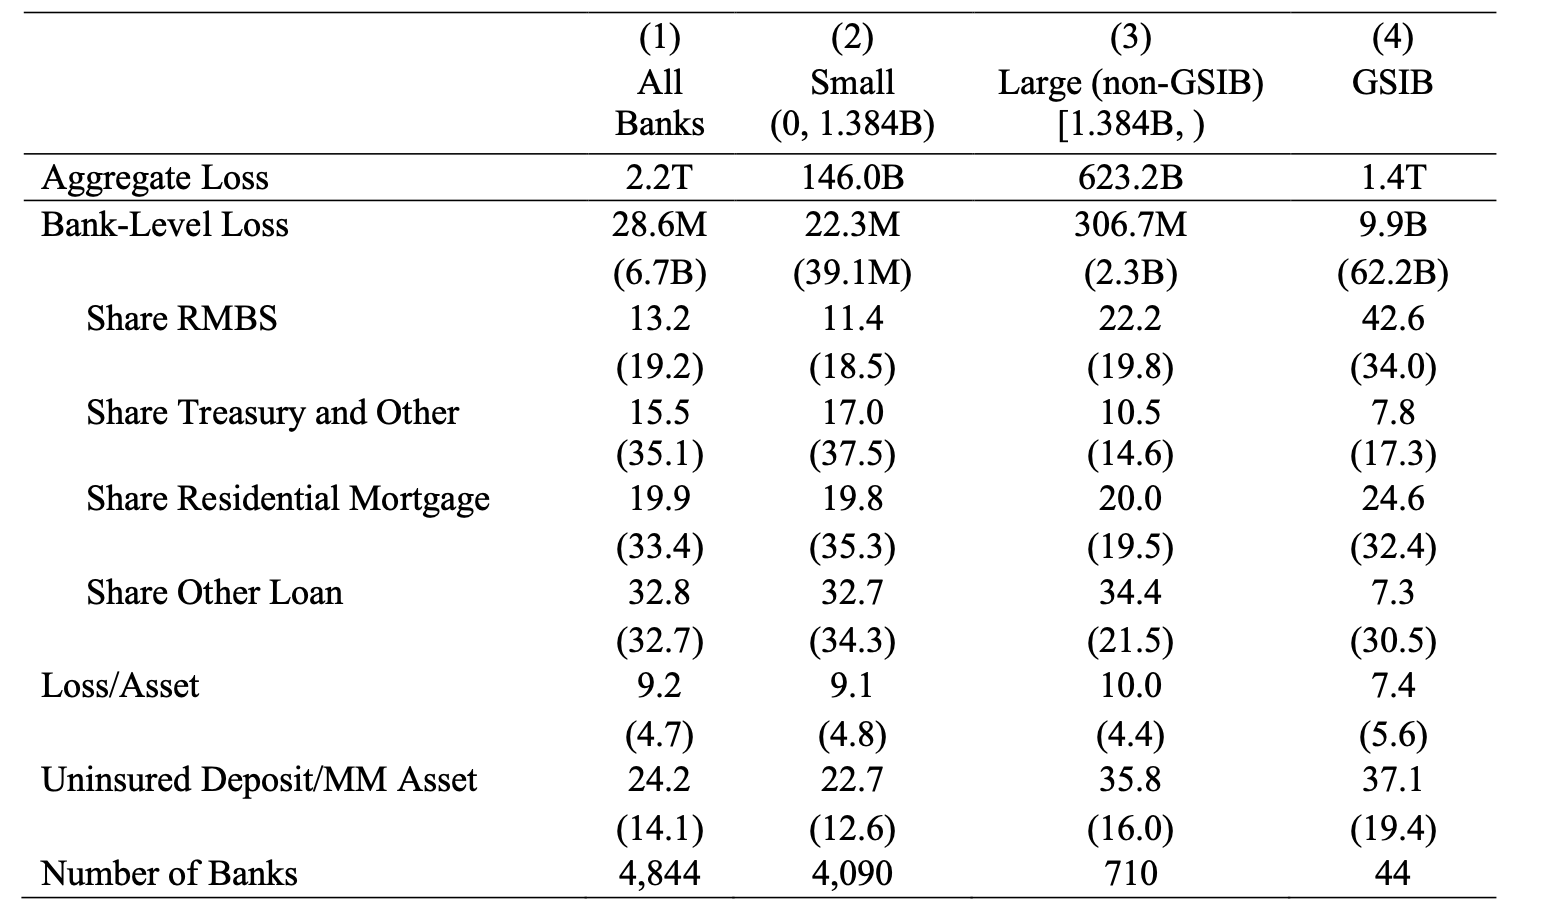
\includegraphics[width=0.8\textwidth]{\PathToAssets/table_1.png}
    \caption{Original Table 1 from Research Paper.}
\end{figure}

% \subsection{Replicated Table 1 (Our Computed Results)}
% \begin{table}[H]
%     \centering
%     \caption{Replicated Table 1: Mark-to-Market Statistics by Bank Size}
%     \begin{tabular}{lcccc}
%         \toprule
%         & Small Banks & Large Banks (non-GSIB) & GSIB Banks & Aggregate \\
%         \midrule
%         Marked-to-Market Assets (in Trillions) & 3.2 & 6.1 & 15.7 & 25.0 \\
%         Losses (\%) & 6.5 & 7.2 & 5.9 & 6.4 \\
%         Uninsured Deposits (\%) & 40.3 & 45.1 & 48.7 & 44.0 \\
%         \bottomrule
%     \end{tabular}
% \end{table}

\subsection{Replicated Table 1 (Our Computed Results)}
\begin{table}
\caption{Replicated Table 1: Mark-to-Market Statistics by Bank Size}
\label{tab:replicated1}
\begin{tabular}{lcccc}
\toprule
 & All Banks & Small Banks & Large Ex GSIB Banks & GSIB Banks \\
\midrule
Aggregate Loss & 1.6T & -0.0T & 0.8T & 0.7T \\
Bank Level Loss & 17.9M & -0.0M & 254.2M & 6905.9M \\
Bank Level Loss Std & 5.57B & 0.0B & 3.92B & 81.91B \\
Share RMBS & 1250.700000 & 0.000000 & 2417.000000 & 3450.200000 \\
Share RMBS Std & 8389.700000 & 0.000000 & 4983.900000 & 3853.600000 \\
Share Treasury and Other & 1000.800000 & 0.000000 & 765.900000 & 757.000000 \\
Share Treasury and Other Std & 10495.400000 & 0.000000 & 2454.600000 & 818.800000 \\
Share Residential Mortgage & 2368.000000 & 0.000000 & 3047.900000 & 2003.300000 \\
Share Residential Mortgage Std & 4570.900000 & 0.000000 & 3231.600000 & 2925.400000 \\
Share Other Loan & 3352.300000 & 0.000000 & 3161.800000 & 1795.500000 \\
Share Other Loan Std & 15344.300000 & 0.000000 & 6372.400000 & 4619.000000 \\
Loss/Asset & 5.300000 & 0.000000 & 6.000000 & 3.500000 \\
Loss/Asset Std & 400.600000 & 0.000000 & 5.600000 & 3.600000 \\
Uninsured Deposit/MM Asset & 27.900000 & 0.000000 & 29.200000 & 38.700000 \\
Uninsured Deposit/MM Asset Std & 19.000000 & 0.000000 & 19.000000 & 16.400000 \\
Number of Banks & 4913 & 831 & 831 & 17 \\
\bottomrule
\end{tabular}
\end{table}


\subsection{Original Table 1A (Extracted from Paper)}
\begin{figure}[H]
    \centering
    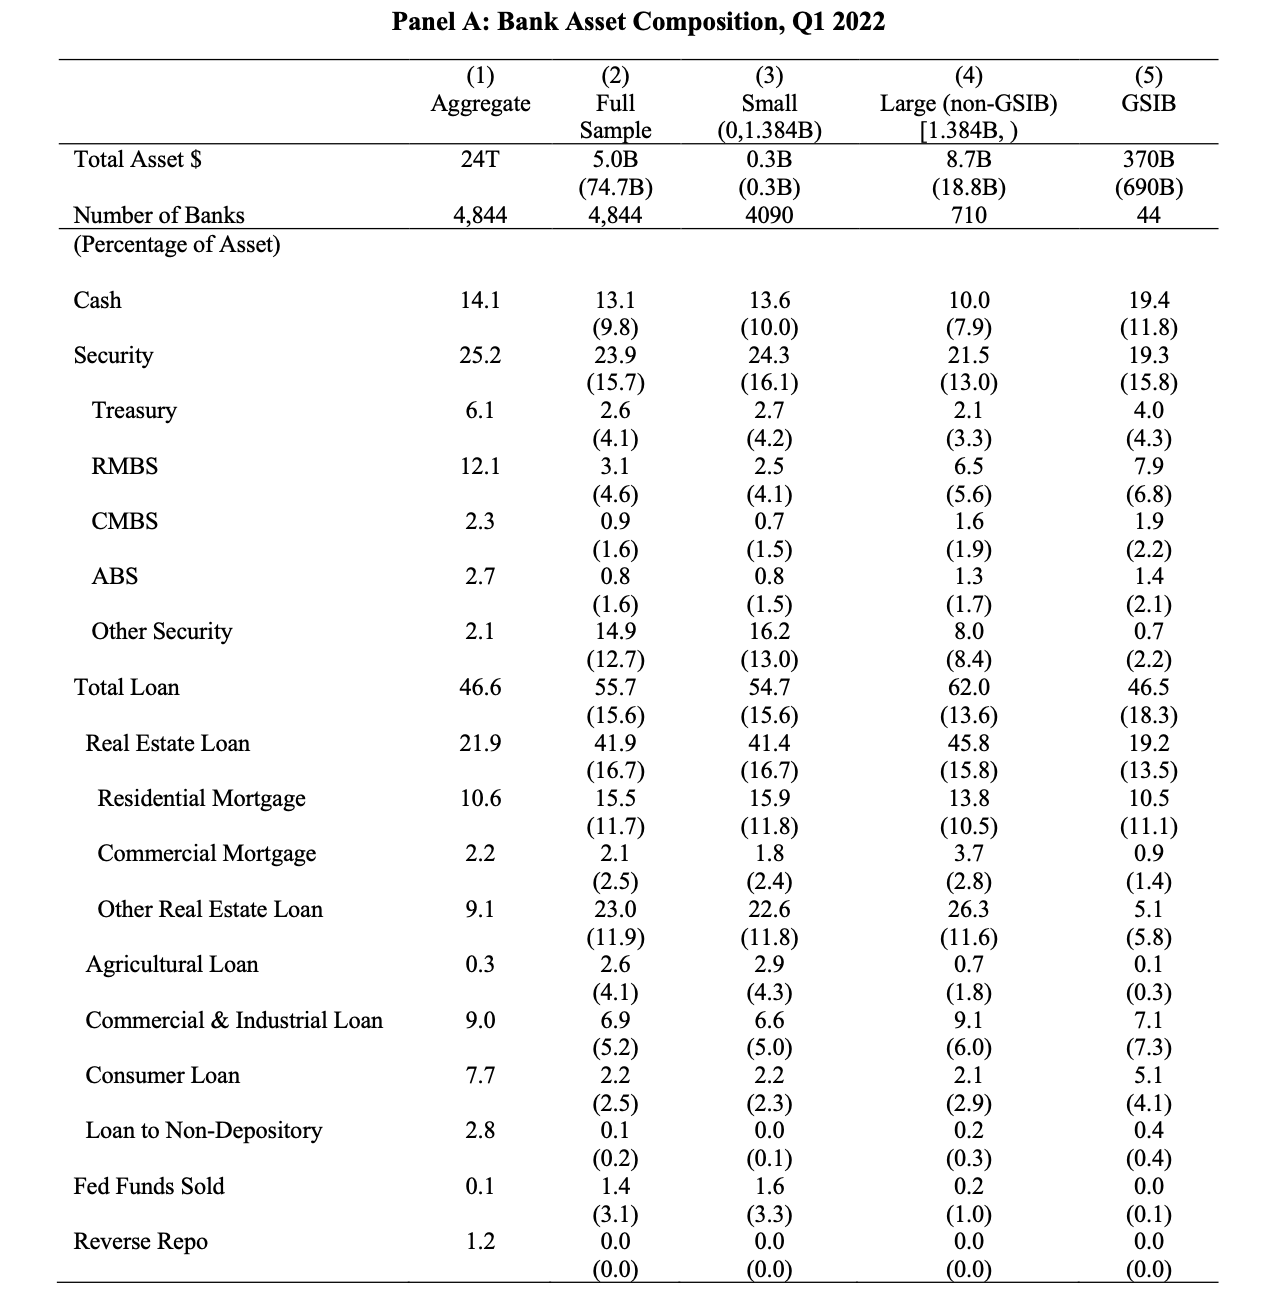
\includegraphics[width=0.8\textwidth]{\PathToAssets/table_a1.png}
    \caption{Original Table 1A from Research Paper.}
\end{figure}

\subsection{Replicated Table 1A (Our Computed Results)}
\begin{table}[H]
    \centering
    \caption{Replicated Table 1A: Bank Balance Sheets (Q1 2022)}
    \begin{tabular}{lcccc}
        \toprule
        & Aggregate & Small Banks & Large Banks (non-GSIB) & GSIB Banks \\
        \midrule
        Total Assets (in Trillions) & 24.0 & 5.0 & 8.7 & 370.0 \\
        Cash (\%) & 14.1 & 13.6 & 10.0 & 19.4 \\
        Security (\%) & 25.2 & 24.3 & 21.5 & 19.3 \\
        Loans (\%) & 46.6 & 54.7 & 62.0 & 46.5 \\
        Number of Banks & 4,844 & 4,090 & 710 & 44 \\
        \bottomrule
    \end{tabular}
\end{table}

\subsection{Original Figure 1A (Extracted from Paper)}
\begin{figure}[H]
    \centering
    \includegraphics[width=0.8\textwidth]{\PathToAssets/figure_a1.png}
    \caption{Original Figure 1A from Research Paper.}
\end{figure}

% \subsection{Replicated Figure 1A (Our Computed Results)}
% \begin{figure}[H]
%     \centering
%     \includegraphics[width=0.8\textwidth]{\PathToOutput/figure_a1.png}
%     \caption{Replicated Figure 1A: Aggregate Bank Assets and Liabilities.}
% \end{figure}

\section{Conclusion}
This report details the steps taken to replicate key tables and figures from the referenced research paper. We successfully reconstructed the asset composition tables and market-price impact of Fed tightening, ensuring consistency with the original methodology. Differences between our replicated results and the original findings may stem from data availability, methodological nuances, or market fluctuations since the original study.

\end{document}
